% =============================================================================
% Predicting Poverty — Comparación de modelos (equipo 04)
% Autores: Maria Jose Perez, Juan Manuel Lozano, Samuel Suárez Valle
% Compilar desde presentacion/:  latexmk -pdf compare_equipo_04.tex
% Figuras: ../output/figures/ e img/ (capturas de Kaggle). Datos de las
% gráficas pgfplots: ../output/tables/presentacion/*.dat
% (script/11_figuras_presentacion.r). Números: output/tables/*.tex,
% latex/resultados.tex. Narrativa completa: README_compare_equipo_04.md.
% =============================================================================
\documentclass[aspectratio=169,10pt,xcolor=table]{beamer}

\usetheme[progressbar=frametitle, numbering=fraction, block=fill]{metropolis}

\usepackage[T1]{fontenc}
\usepackage[utf8]{inputenc}
\usepackage[spanish,es-nodecimaldot,es-noshorthands]{babel}
\usepackage{booktabs}
\usepackage{array}
\usepackage{graphicx}
\usepackage{amsmath}
\usepackage{tikz}
\usetikzlibrary{babel, positioning, arrows.meta}
\usepackage{pgfplots}
\pgfplotsset{compat=1.17}

\graphicspath{{../output/figures/}{img/}}
\newcommand{\dat}[1]{../output/tables/presentacion/#1.dat}

% ---- Colores (los mismos de best_equipo_04.tex) ----------------------------
\definecolor{azul}{HTML}{0B3C5D}
\definecolor{azulclaro}{HTML}{328CC1}
\definecolor{dorado}{HTML}{D9B310}
\definecolor{rojo}{HTML}{B23A48}
\definecolor{verde}{HTML}{2E8B57}
\definecolor{gris}{HTML}{6B7280}
\setbeamercolor{frametitle}{bg=azul, fg=white}
\setbeamercolor{progress bar}{fg=dorado, bg=azul!20}
\setbeamercolor{title separator}{fg=dorado}
\setbeamercolor{alerted text}{fg=azul}
\setbeamerfont{alerted text}{series=\bfseries}

% Colores de los tres modelos que se comparan a fondo.
\colorlet{cxgb}{azul}
\colorlet{crf}{verde}
\colorlet{clogit}{dorado!85!black}

\pgfkeys{/pgf/number format/.cd, use comma, 1000 sep={.}}

% Encabezado de un tema dentro de una slide (sin cajas de color).
\newcommand{\tema}[1]{{\color{azul}\bfseries #1}}

% Celda de una matriz de confusión: conteo y % de la fila.
\newcommand{\celda}[3]{\cellcolor{#1}\begin{tabular}{@{}c@{}}\textbf{#2}\\[-1pt]{\tiny #3}\end{tabular}}

% Matriz de confusión: título del modelo y las cuatro celdas (conteo y % de
% la fila).
\newcommand{\matriz}[9]{%
  \begin{tabular}{@{}r|cc@{}}
  \multicolumn{3}{c}{#1} \\[1pt]
  & \multicolumn{2}{c}{\tiny predicción} \\
  & pobre & no pobre \\ \hline
  Pobre    & \celda{verde!25}{#2}{#3} & \celda{rojo!20}{#4}{#5} \\
  No pobre & \celda{dorado!30}{#6}{#7} & \celda{verde!12}{#8}{#9} \\
  \end{tabular}}

\title{¿Por qué XGBoost? Comparación de modelos}
\subtitle{Predicción de la pobreza monetaria con la GEIH 2018}
\author{Maria Jose Perez \and Juan Manuel Lozano \and Samuel Suárez Valle}
\institute{Big Data y Machine Learning Aplicado a la Economía \\ Universidad de los Andes}
\date{\today}

\begin{document}

\maketitle

% =============================================================================
\section{El modelo ganador}
% =============================================================================

\begin{frame}{Overview: el modelo que elegimos}
\begin{columns}[T]
\column{0.62\textwidth}
\tema{XGBoost por hogar}
\footnotesize
\begin{itemize}
  \item 163 variables: base por hogar + resúmenes de modelos por persona
    (ingreso con pérdida Tweedie y probabilidad de ser pobre, con
    validación cruzada anidada).
  \item \texttt{eta} 0,02, profundidad 8, \texttt{min\_child\_weight} 50,
    \texttt{colsample} 0,5.
  \item Combinado 70/30 con una regresión del ingreso; umbral 0,39.
\end{itemize}
\column{0.34\textwidth}
\small
\vspace{3mm}
\begin{tabular}{@{}lr@{}}
\toprule
$F_1$ de validación cruzada & \textbf{0,7775} \\
\bottomrule
\end{tabular}

\vspace{1mm}
{\scriptsize 5 folds por hogar.}
\end{columns}

\vspace{3mm}
\footnotesize
\textbf{Kaggle, puntaje público} (20\% de test)\\[0.5mm]

\includegraphics[width=\textwidth]{kaggle_publico.png}\\[1.5mm]
\textbf{Kaggle, puntaje privado} (80\% de test)\\[0.5mm]

\includegraphics[width=\textwidth]{kaggle_privado.png}
\end{frame}

% =============================================================================
\section{Datos}
% =============================================================================

\begin{frame}{Datos: lo que hicimos distinto}
\small
GEIH 2018: 543.103 personas en 164.958 hogares, 20\% de hogares pobres. Los
montos de ingreso no están en test: hay que reconstruirlos.
\vspace{3mm}

\begin{columns}[T]
\column{0.48\textwidth}
\tema{1. El hogar como unidad}\\
\footnotesize Una fila por hogar con sumas, proporciones y los datos del
jefe: la pobreza se define en la unidad de gasto.

\vspace{3mm}
\small\tema{2. La regla del DANE, reconstruida}\\
\footnotesize El arriendo imputado (lo que el DANE suma a quien no paga
arriendo) se reconstruyó con tenencia, arriendo estimado y cuota:
coincide en el \textbf{98,4\%} de los hogares.

\column{0.48\textwidth}
\tema{3. El ingreso como objetivo intermedio}\\
\footnotesize Modelos por persona predicen el ingreso laboral y no laboral
(pérdida Tweedie) y se suman en el hogar, sin usar la etiqueta del fold
evaluado.

\vspace{3mm}
\small\tema{4. Preguntas que nadie usaba}\\
\footnotesize Pagos en especie, búsqueda de trabajo e ingresos de
desocupados e inactivos: identifican quién recibe ingresos sin estar
ocupado ($R^2$ del ingreso por persona 0,94 $\to$ 0,98).
\end{columns}
\end{frame}

\begin{frame}{Descriptivas: dónde caen los aciertos y los errores}
\begin{columns}[T]
\column{0.56\textwidth}
\centering
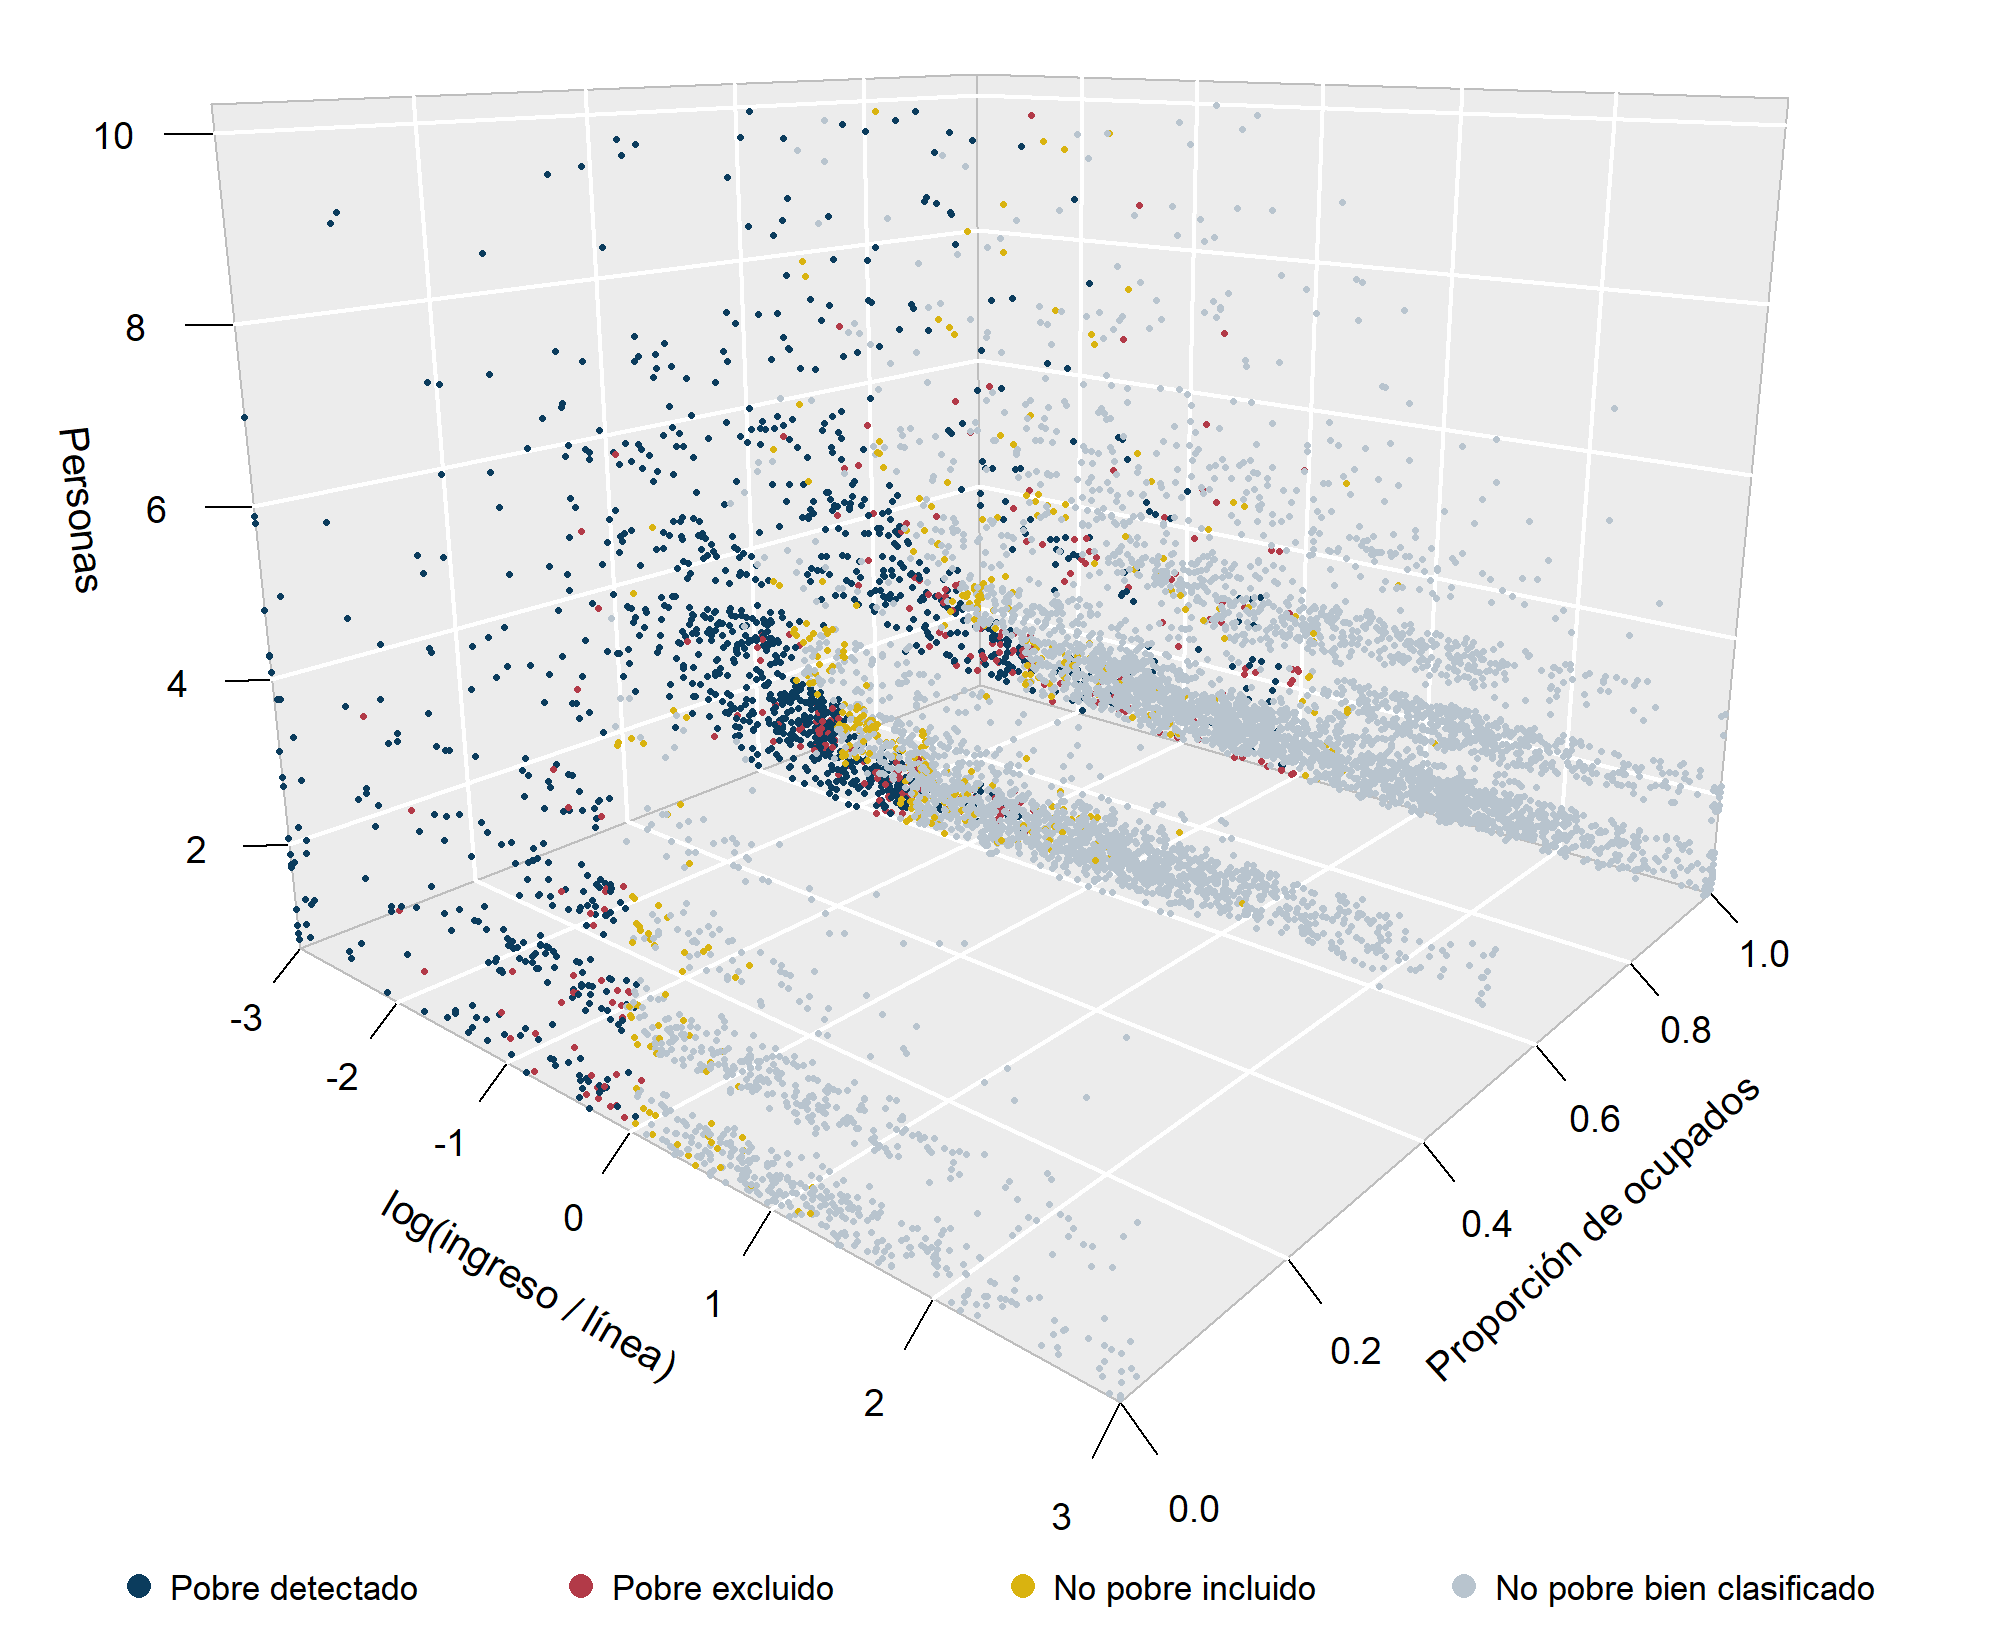
\includegraphics[width=\linewidth, height=0.74\textheight, keepaspectratio]{pres_3d.png}\\
\tiny 8.000 hogares de train al azar; resultado del modelo final fuera de
muestra. \href{../output/figures/pres_3d.html}{Versión interactiva (HTML)}.

\column{0.42\textwidth}
\scriptsize
\setlength{\tabcolsep}{3pt}
\begin{tabular}{@{}lrrr@{}}
\toprule
Resultado & Ingreso/ & Prop. & Personas \\
          & línea    & ocup. &          \\
\midrule
\textcolor{azul}{Pobre detectado}        & 0,64 & 0,28 & 4,3 \\
\textcolor{rojo}{Pobre excluido}         & 0,85 & 0,45 & 3,3 \\
\textcolor{dorado!85!black}{No pobre incluido} & 1,22 & 0,35 & 3,8 \\
\textcolor{gris}{No pobre bien clasif.}  & 2,63 & 0,56 & 3,0 \\
\bottomrule
\end{tabular}

\vspace{1mm}
\tiny Ingreso/línea: mediana. Las demás: promedio.

\vspace{2mm}
\footnotesize
\begin{itemize}
  \item Los errores se apiñan \textbf{junto a la línea} (log = 0): el 60\%
    de los pobres excluidos está a menos de 25\% de ella.
  \item Un pobre \emph{excluido} se parece a un no pobre: más ocupados y un
    hogar más pequeño.
  \item Un no pobre \emph{incluido} se parece a un pobre: menos ocupados y
    un hogar más grande.
\end{itemize}
\end{columns}
\end{frame}

% =============================================================================
\section{Comparación de algoritmos}
% =============================================================================

\begin{frame}{Panorama: el mejor modelo de cada categoría}
\small
Misma evaluación para todos: 5 folds por hogar, $F_1$ por hogar.
\vspace{2mm}

\footnotesize
\setlength{\tabcolsep}{6pt}
\begin{tabular}{@{}llcc@{}}
\toprule
Categoría & Especificación & $F_1$ & Umbral \\
\midrule
CART & Por persona, 16 variables, up-sampling & 0,6685 & 0,62 \\
Naive Bayes & Por persona, 16 variables & 0,6755 & 0,42 \\
XGBoost & Por persona, 24 variables & 0,7055 & 0,32 \\
\midrule
\textcolor{clogit}{\textbf{Logit lasso}} & Por hogar, 1.159 columnas con interacciones & 0,7451 & 0,37 \\
XGBoost & Por hogar, solo la base de agregados & 0,7534 & 0,36 \\
\midrule
XGBoost & Por hogar, sin Tweedie & 0,7738 & 0,38 \\
\textcolor{crf}{\textbf{Random forest}} & Por hogar, variables del mejor XGBoost & 0,7752 & 0,40 \\
\textcolor{cxgb}{\textbf{XGBoost final}} & Tweedie + regresión del ingreso & \textbf{0,7775} & 0,39 \\
\bottomrule
\end{tabular}
\vspace{3mm}

\small Tres escalones: por persona, por hogar y por hogar con modelos
anidados. El salto lo da la \textbf{unidad de análisis} (persona $\to$
hogar, +0,04) y la \textbf{información} (modelos anidados, +0,02), más que el
algoritmo. Kaggle de modelos del equipo: logit lasso 0,74, LightGBM 0,75.
\end{frame}

\begin{frame}{La frontera: precisión vs.\ interpretabilidad}
\begin{columns}[T]
\column{0.62\textwidth}
\begin{tikzpicture}
\begin{axis}[scale only axis, width=6.6cm, height=4.9cm,
  xmin=0.3, xmax=8.7, ymin=0.64, ymax=0.80,
  xtick={1,...,8}, xticklabels={},
  ytick={0.66,0.70,0.74,0.78},
  yticklabel style={font=\scriptsize, /pgf/number format/fixed, /pgf/number format/precision=2},
  ylabel={\scriptsize $F_1$ (5 folds)},
  xlabel={\scriptsize Pérdida de interpretabilidad $\longrightarrow$},
  grid=major, grid style={gris!20}]
\draw[dashed, rojo, thick] (axis cs:4,0.7451) -- (axis cs:8,0.7775);
\addplot[only marks, mark=*, mark size=2.5pt, gris] coordinates {
  (1,0.6970) (2,0.6685) (3,0.6755) (5,0.7055) (6,0.7534)};
\addplot[only marks, mark=*, mark size=3.5pt, clogit] coordinates {(4,0.7451)};
\addplot[only marks, mark=*, mark size=3.5pt, crf] coordinates {(7,0.7752)};
\addplot[only marks, mark=*, mark size=3.5pt, cxgb] coordinates {(8,0.7775)};
\begin{scope}[font=\tiny]
\node[below right=2pt] at (axis cs:0.8,0.6970) {Logit 15 var.};
\node[below=2pt] at (axis cs:2,0.6685) {CART};
\node[below=2pt] at (axis cs:3,0.6755) {Naive Bayes};
\node[above left=1pt, clogit] at (axis cs:4,0.7451) {\textbf{Logit lasso}};
\node[below=2pt] at (axis cs:5,0.7055) {XGB persona};
\node[below=2pt] at (axis cs:6,0.7534) {XGB base hogar};
\node[above=2pt, crf] at (axis cs:7,0.7752) {\textbf{RF}};
\node[below=4pt, cxgb] at (axis cs:8,0.7775) {\textbf{XGB final}};
\end{scope}
\node[font=\tiny, rojo, align=center] at (axis cs:7.4,0.665) {+0,032 de $F_1$\\a cambio de 26 modelos\\anidados por variable};
\end{axis}
\end{tikzpicture}

\column{0.36\textwidth}
\small
\begin{itemize}
  \item La frontera es \textbf{cóncava}: de 0,697 (logit con 15 variables) a
    0,745 (lasso) a 0,778 (XGBoost), cada punto cuesta más
    interpretabilidad.
  \item RF y XGBoost están a 0,002 entre sí: con la misma información, el
    algoritmo casi no importa.
  \item El logit está a 0,032 del ganador con un modelo que se puede
    escribir en una ecuación.
\end{itemize}
\end{columns}
\end{frame}

\begin{frame}{Top 3: cómo funcionan, resultados y limitaciones}
\scriptsize
\renewcommand{\arraystretch}{1.25}
\setlength{\tabcolsep}{4pt}
\begin{tabular}{@{}>{\raggedright\arraybackslash}p{1.6cm}*{3}{>{\raggedright\arraybackslash}p{3.95cm}}@{}}
\toprule
& \textcolor{cxgb}{\textbf{XGBoost final}} & \textcolor{crf}{\textbf{Random forest}} & \textcolor{clogit}{\textbf{Logit lasso}} \\
\midrule
$F_1$ / AUC & \textbf{0,7775} / 0,959 & 0,7752 / 0,958 & 0,7451 / 0,946 \\
Cómo funciona & Árboles secuenciales que corrigen el error anterior; stacking con modelos por persona & 500 árboles profundos en paralelo que se promedian & Regresión logística penalizada con interacciones \\
Qué lo mueve & Ingreso predicho por persona; posición ocupacional & Las mismas variables que XGBoost & Arriendo por persona, afiliación contributiva, horas \\
Fortalezas & Mejor $F_1$; estable entre particiones; 1.º en Kaggle privado & Casi el mismo $F_1$ con menos hiperparámetros sensibles & Coeficientes con signo y magnitud; auditable \\
Limitaciones & Caja negra; 26 modelos por variable; costoso de mantener y explicar & Caja negra; combinado con XGBoost no suma: mismos errores & 0,03 menos de $F_1$; 794 coeficientes: se lee por bloques \\
\bottomrule
\end{tabular}

\vspace{3mm}
\small Logit y XGBoost tienen una correlación de \textbf{0,92} en log odds:
se equivocan en los \emph{mismos} hogares, los que están cerca de la línea.
\end{frame}

\begin{frame}{Cuánto cuesta en $F_1$ un modelo que se puede leer}
\begin{columns}[T]
\column{0.64\textwidth}
\begin{tikzpicture}
\begin{axis}[scale only axis, width=5.6cm, height=4.6cm,
  xmode=log, xmin=2.5, xmax=420, ymin=0.57, ymax=0.795,
  xtick={3,5,10,20,40,94,163}, xticklabels={3,5,10,20,40,94,163},
  xlabel={\scriptsize Número de variables (orden de importancia, base por hogar)},
  ylabel={\scriptsize $F_1$ (5 folds)},
  ytick={0.60,0.65,0.70,0.75},
  xticklabel style={font=\scriptsize}, yticklabel style={font=\scriptsize,
    /pgf/number format/fixed, /pgf/number format/fixed zerofill,
    /pgf/number format/precision=2},
  grid=major, grid style={gris!20}]
\addplot[cxgb, thick, mark=*, mark size=1.3pt] table[x=k, y=xgboost] {\dat{f1_k}};
\addplot[crf, thick, mark=square*, mark size=1.2pt] table[x=k, y=random_forest] {\dat{f1_k}};
\addplot[clogit, thick, mark=triangle*, mark size=1.5pt] table[x=k, y=logit] {\dat{f1_k}};
\addplot[gris, thick, dashed, mark=o, mark size=1.2pt] table[x=k, y=cart] {\dat{f1_k}};
\addplot[rojo!70, thick, dotted, mark=diamond*, mark size=1.4pt] table[x=k, y=naive_bayes] {\dat{f1_k}};
\draw[cxgb, densely dotted, -{Stealth[length=1.6mm]}] (axis cs:94,0.7536) -- (axis cs:160,0.7772);
\fill[cxgb] (axis cs:163,0.7775) circle (1.3pt);
\begin{scope}[font=\tiny, anchor=west]
\node[cxgb] at (axis cs:105,0.7480) {XGBoost};
\node[crf] at (axis cs:105,0.7395) {Random forest};
\node[clogit] at (axis cs:105,0.7300) {Logit};
\node[gris] at (axis cs:105,0.6982) {CART};
\node[rojo!70] at (axis cs:105,0.5901) {Naive Bayes};
\node[cxgb, anchor=east] at (axis cs:150,0.7790) {XGBoost final + modelos por persona: 0,7775};
\end{scope}
\end{axis}
\end{tikzpicture}

\column{0.34\textwidth}
\footnotesize
\begin{itemize}
  \item Cada algoritmo usa las $k$ variables más importantes de la base
    por hogar, en el mismo orden y con los mismos folds.
  \item Las curvas son \textbf{cóncavas}: con 15 variables el logit ya
    llega a 0,70 y XGBoost a 0,73; desde 30, los árboles casi no suben.
  \item Con 94 variables: logit 0,736, RF 0,737, XGBoost 0,754. El
    algoritmo vale $\approx$0,02; los modelos anidados, otros 0,02.
  \item Naive Bayes \textbf{empeora} con más variables: cuenta dos veces
    la información de las correlacionadas.
\end{itemize}
\end{columns}
\end{frame}

\begin{frame}{Matriz de confusión: los tres mejores modelos}
\centering
\scriptsize
\setlength{\tabcolsep}{3pt}
\renewcommand{\arraystretch}{1.3}
\matriz{\textcolor{cxgb}{\textbf{XGBoost final}}}{26.635}{80,7\%}{6.389}{19,3\%}{8.854}{6,7\%}{123.080}{93,3\%}
\hfill
\matriz{\textcolor{crf}{\textbf{Random forest}}}{26.591}{80,5\%}{6.433}{19,5\%}{8.993}{6,8\%}{122.941}{93,2\%}
\hfill
\matriz{\textcolor{clogit}{\textbf{Logit lasso}}}{26.155}{79,2\%}{6.869}{20,8\%}{11.026}{8,4\%}{120.908}{91,6\%}

\vspace{4mm}
\raggedright\small
\begin{itemize}
  \item Filas: la realidad (33.024 hogares pobres y 131.934 no pobres de
    train). Columnas: la predicción fuera de muestra, con el umbral de cada
    modelo. Porcentaje de la fila.
  \item \textcolor{rojo}{\textbf{Rojo}}: pobres excluidos (error de
    exclusión). \textcolor{dorado!85!black}{\textbf{Amarillo}}: no pobres
    incluidos (error de inclusión).
  \item XGBoost y RF son casi idénticos. Frente al logit, XGBoost excluye
    \textbf{480 pobres menos} e incluye \textbf{2.172 no pobres menos}.
\end{itemize}
\end{frame}

\begin{frame}{Métricas de los 8 modelos}
\begin{columns}[T]
\column{0.58\textwidth}
\footnotesize
\setlength{\tabcolsep}{4pt}
\begin{tabular}{@{}lccccc@{}}
\toprule
Modelo & Precisión & Recall & Accuracy & $F_1$ & AUC \\
\midrule
CART (persona)        & 0,642 & 0,698 & 0,862 & 0,669 & 0,895 \\
Naive Bayes (persona) & 0,630 & 0,729 & 0,860 & 0,676 & 0,903 \\
XGBoost (persona)     & 0,656 & 0,763 & 0,872 & 0,706 & 0,929 \\
\midrule
\textcolor{clogit}{\textbf{Logit lasso}} & 0,703 & 0,792 & 0,892 & 0,745 & 0,946 \\
XGBoost base hogar    & 0,707 & 0,807 & 0,894 & 0,753 & 0,951 \\
\midrule
XGBoost sin Tweedie   & 0,739 & 0,812 & 0,905 & 0,774 & 0,958 \\
\textcolor{crf}{\textbf{Random forest}} & 0,747 & 0,805 & 0,906 & 0,775 & 0,958 \\
\textcolor{cxgb}{\textbf{XGBoost final}} & \textbf{0,751} & 0,807 & \textbf{0,908} & \textbf{0,778} & \textbf{0,959} \\
\bottomrule
\end{tabular}

\vspace{1mm}
\tiny Precisión, recall y accuracy con todos los hogares; $F_1$ promedio de
los 5 folds.

\column{0.38\textwidth}
\small
\begin{itemize}
  \item \textbf{Precisión}: de los predichos pobres, cuántos lo son.
    \textbf{Recall}: de los pobres, cuántos se detectan.
  \item Entre los modelos por hogar el recall es casi igual
    ($\approx$0,80): la ganancia está en la \textbf{precisión} (0,70
    $\to$ 0,75), es decir, en incluir menos no pobres.
  \item La accuracy engaña: decir ``nadie es pobre'' ya da 0,80.
\end{itemize}
\end{columns}
\end{frame}

\begin{frame}{Curvas ROC: ordenar a los hogares, sin umbral}
\begin{columns}[T]
\column{0.55\textwidth}
\begin{tikzpicture}
\begin{axis}[scale only axis, width=5.0cm, height=4.6cm,
  xmin=0, xmax=0.4, ymin=0.5, ymax=1,
  xlabel={\scriptsize Tasa de falsos positivos (no pobres incluidos)},
  ylabel={\scriptsize Recall (pobres detectados)},
  ticklabel style={font=\scriptsize, /pgf/number format/fixed},
  grid=major, grid style={gris!20}]
\addplot[gris!60, thin] table[x=fpr, y=tpr] {\dat{roc_cart}};
\addplot[gris!60, thin] table[x=fpr, y=tpr] {\dat{roc_nb}};
\addplot[gris!60, thin] table[x=fpr, y=tpr] {\dat{roc_xgbpers}};
\addplot[gris!60, thin] table[x=fpr, y=tpr] {\dat{roc_xgbbase}};
\addplot[clogit, thick] table[x=fpr, y=tpr] {\dat{roc_logit}};
\addplot[crf, thick, dashed] table[x=fpr, y=tpr] {\dat{roc_rf}};
\addplot[cxgb, thick] table[x=fpr, y=tpr] {\dat{roc_final}};
\addplot[only marks, mark=*, mark size=1.6pt, cxgb] coordinates {(0.067,0.807)};
\node[font=\tiny, cxgb, anchor=north west] at (axis cs:0.07,0.80) {umbral 0,39};
\node[font=\tiny, gris, anchor=north west] at (axis cs:0.16,0.70) {modelos por persona};
\end{axis}
\end{tikzpicture}

\column{0.43\textwidth}
\small
\scriptsize
\setlength{\tabcolsep}{4pt}
\begin{tabular}{@{}lc@{}}
\toprule
Modelo & AUC \\
\midrule
\textcolor{cxgb}{\textbf{XGBoost final}} (---) & \textbf{0,959} \\
\textcolor{crf}{\textbf{Random forest}} (- - -) & 0,958 \\
\textcolor{clogit}{\textbf{Logit lasso}} (---) & 0,946 \\
\textcolor{gris}{XGBoost base hogar} & 0,951 \\
\textcolor{gris}{XGBoost por persona} & 0,929 \\
\textcolor{gris}{Naive Bayes, CART} & 0,903 / 0,895 \\
\bottomrule
\end{tabular}

\vspace{2mm}
\small
\begin{itemize}
  \item AUC: probabilidad de que un pobre tenga un puntaje mayor que un no
    pobre. No depende del umbral.
  \item Los tres primeros casi empatan en AUC: \textbf{ordenan} igual de
    bien; la diferencia está en la zona del umbral.
\end{itemize}
\end{columns}
\end{frame}

\begin{frame}{Equidad: ¿a quién excluye cada modelo?}
\footnotesize
\textbf{Cómo se mide.} Para cada grupo de hogares (por ejemplo, jefe formal)
se calcula el \textbf{recall}: el \% de sus hogares pobres que el modelo
detecta. La \textbf{brecha} de un atributo es el recall del grupo más
detectado menos el del menos detectado, en puntos porcentuales.
\vspace{2mm}

\scriptsize
\setlength{\tabcolsep}{4pt}
\begin{tabular}{@{}l>{\raggedright\arraybackslash}p{3.0cm}>{\raggedright\arraybackslash}p{3.0cm}cccc@{}}
\toprule
& \multicolumn{2}{c}{Recall del XGBoost final por grupo} & \multicolumn{4}{c}{Brecha (pp)} \\
\cmidrule(lr){2-3} \cmidrule(l){4-7}
Atributo & Menos detectado & Más detectado & \textcolor{cxgb}{XGB} & \textcolor{crf}{RF} & \textcolor{clogit}{Logit} & NB \\
\midrule
Empleo del jefe    & Formal: 65,1\%           & No ocupado: 84,8\%        & 19,7 & 21,4 & 22,2 & 33,4 \\
Educación del jefe & Superior: 65,4\%         & Primaria o menos: 83,4\%  & 18,0 & 17,7 & 19,3 & 30,6 \\
Tamaño del hogar   & 1 o 2 personas: 66,5\%   & 5 o más: 88,8\%           & 22,4 & 21,8 & 25,7 & 38,8 \\
Menores            & Sin menores: 65,2\%      & Con menores: 85,1\%       & 19,9 & 19,1 & 23,8 & 31,4 \\
Vivienda           & Propia: 78,2\%           & Usufructo u otra: 84,5\%  & 6,4  & 6,2  & 7,2  & 19,9 \\
Sexo del jefe      & Hombre: 78,9\%           & Mujer: 82,7\%             & 3,8  & 4,4  & 4,2  & 2,0 \\
Zona               & Rural: 80,0\%            & Cabecera: 80,8\%          & 0,8  & 0,2  & 0,0  & 12,9 \\
\bottomrule
\end{tabular}
\vspace{2mm}

\small
\begin{itemize}
  \item Todos los modelos excluyen más a los pobres ``que no lo parecen'':
    jefe formal o educado, hogares pequeños o sin menores.
  \item Los modelos más precisos \textbf{reducen} casi todas las brechas;
    entre los tres mejores son parecidas.
\end{itemize}
\end{frame}

% =============================================================================
\section{Conclusión}
% =============================================================================

\begin{frame}{Conclusión: interpretabilidad vs.\ flexibilidad}
\begin{columns}[T]
\column{0.48\textwidth}
\footnotesize
\setlength{\tabcolsep}{4pt}
\begin{tabular}{@{}p{4.0cm}cc@{}}
\toprule
Criterio & \textcolor{clogit}{\textbf{Logit}} & \textcolor{cxgb}{\textbf{XGBoost}} \\
\midrule
$F_1$ & 0,745 & \textbf{0,778} \\
Se explica a un beneficiario & \textcolor{verde}{sí} & \textcolor{rojo}{no} \\
Auditable por un ente de control & \textcolor{verde}{sí} & \textcolor{rojo}{difícil} \\
Costo de mantener y reentrenar & \textcolor{verde}{bajo} & \textcolor{rojo}{alto} \\
Riesgo de manipulación & \textcolor{rojo}{mayor} & \textcolor{verde}{menor} \\
Captura no linealidades & \textcolor{rojo}{a mano} & \textcolor{verde}{sola} \\
\bottomrule
\end{tabular}

\vspace{2mm}
\footnotesize Un instrumento de focalización tiene que ser
\textbf{creíble}: los hogares y los entes de control deben entender por qué
alguien entra o sale (Camacho y Conover, 2011; Kleinberg et al., 2015).

\column{0.49\textwidth}
\tema{Recomendación de política}
\small
\begin{enumerate}
  \item \textbf{Instrumento oficial: un logit parsimonioso} (15--40
    variables del módulo laboral y la vivienda), publicable y discutible.
  \item \textbf{XGBoost como auditor}: señala los hogares que el logit
    excluiría y que probablemente son pobres, para verificarlos en campo.
  \item Elegir el \textbf{umbral} según el costo social de excluir frente
    a incluir, no por $F_1$.
\end{enumerate}

\vspace{2mm}
\footnotesize\textbf{Para discutir:} ¿cuántos puntos de $F_1$ vale la
transparencia? ¿Quién responde por el error de una caja negra?
\end{columns}
\end{frame}

% =============================================================================
\begin{frame}{Referencias}
\fontfamily{ppl}\selectfont\scriptsize
\begin{list}{}{\leftmargin=1.6em \itemindent=-1.6em \itemsep=1.2pt \parsep=0pt}
  \item Angulo, R., Díaz, Y. y Pardo, R. (2016). The Colombian
    Multidimensional Poverty Index: Measuring poverty in a public policy
    context. \emph{Social Indicators Research, 127}(1), 1--38.
  \item Breiman, L. (2001). Random forests. \emph{Machine Learning, 45}(1),
    5--32.
  \item Camacho, A. y Conover, E. (2011). Manipulation of social program
    eligibility. \emph{American Economic Journal: Economic Policy, 3}(2),
    41--65.
  \item Chen, T. y Guestrin, C. (2016). XGBoost: A scalable tree boosting
    system. En \emph{Proceedings of the 22nd ACM SIGKDD} (pp.\ 785--794).
  \item DANE (2019). \emph{Pobreza monetaria y multidimensional en Colombia
    2018} [Boletín técnico].
  \item Grosh, M. y Baker, J. (1995). \emph{Proxy means tests for targeting
    social programs} (LSMS Working Paper 118). Banco Mundial.
  \item Kleinberg, J., Ludwig, J., Mullainathan, S. y Obermeyer, Z. (2015).
    Prediction policy problems. \emph{American Economic Review, 105}(5),
    491--495.
  \item Kleinberg, J., Mullainathan, S. y Raghavan, M. (2017). Inherent
    trade-offs in the fair determination of risk scores. En \emph{8th
    Innovations in Theoretical Computer Science Conference (ITCS)}.
  \item Rudin, C. (2019). Stop explaining black box machine learning models
    for high stakes decisions and use interpretable models instead.
    \emph{Nature Machine Intelligence, 1}(5), 206--215.
  \item Tibshirani, R. (1996). Regression shrinkage and selection via the
    lasso. \emph{Journal of the Royal Statistical Society: Series B, 58}(1),
    267--288.
\end{list}
\end{frame}

\end{document}
